% TODO:
% http://www.usaco.org/index.php?page=viewproblem2&cpid=972
% https://codeforces.com/gym/102979/problem/G
% http://www.usaco.org/index.php?page=viewproblem2&cpid=698
% https://codeforces.com/contest/1146/problem/G
% https://codeforces.com/contest/1107/problem/E
% https://atcoder.jp/contests/arc104/tasks/arc104_f

\chapter{ম্যাট্রিক্স চেইন মাল্টিপ্লিকেশন এবং ইন্টারভাল ডিপি}

অধ্যায়ের টাইটেল দেখে হয়তো আন্দাজ করতে পারছো এই ধরনের ডিপিতে স্টেট হিসেবে একটা
অ্যারের সাব-অ্যারেকে ডিপিতে স্টেট হিসেবে রাখতে হবে। এই ক্যাটাগরির সবচাইতে
ক্লাসিক্যাল উদাহরণ দিয়ে শুরু করা যাক।

\section{একটি ক্লাসিক্যাল সমস্যা}

\begin{example}[ম্যাট্রিক্স চেইন মাল্টিপ্লিকেশন]
  $n (\le 500)$ টা ম্যাট্রিক্স আছে তোমার কাছে, তোমাকে সবচাইতে কম কস্টে তোমাকে
  এদের গুণফল বের করতে হবে। ফরমালি বলতে গেলে, তোমাকে $n$ টা ম্যাট্রিক্স $A_1,
  A_2,
  \ldots A_n$ এর dimension গুলো, অর্থাৎ, $(N_1, M_1), (N_2, M_2), \ldots,
  (N_n, M_n)$ গুলো দেওয়া আছে, যেখানে $A_i$ এর সাইজ হলো $n_i \times m_i$ আর,
  $M_i = N_{i+1} \, (1 \le i < n)$। তোমাকে বের করতে হবে সবচাইতে কম কতটি লুপ
  চালিয়ে তুমি $A_1 A_2 A_3 \dots A_n$ বের করতে পারবা। $a \times b$ এবং $b
  \times c$ সাইজের দুটি ম্যাটিক্স গুন করার কস্ট $abc$।
\end{example}

\begin{solution}
  তুমি যদি ম্যাট্রিক্স এক্সপোনেন্সিয়েশনের চ্যাপ্টারটি পড়ে থাকো তাহলে জানার
  কথা ম্যাট্রিক্স মাল্টিপ্লিকেশন একটি অ্যাসোসিয়েটিভ অপারেশন। যেমন, $(AB)C$ আর
  $A(BC)$ একই জিনিস, অর্থাৎ, $A$ আর $B$ এর গুণফল বের করে সেটাকে $C$ দিয়ে গুন
  দেওয়া যেই কথা, $A$ কে $B$ আর $C$ এর গুণফল দিয়ে গুন দেওয়াও একই কথা। কিন্তু
  এদের গুনের অর্ডারের উপর $ABC$ বের করতে কত টাইম লাগবে তা নির্ভর করে। যেমন
  ধরো, $A$, $B$ আর $C$ এর সাইজ যথাক্রমে $2 \times 1000$, $1000 \times 3$, $3
  \times 4$। যদি $(AB)C$ করি তাহলে কস্ট কত হয় দেখা যাক। প্রথমে $AB$
  করার জন্য কস্ট হলো $2 \times 1000 \times 3$, এবং এরপর $AB$ ম্যাট্রিক্সটির
  সাইজ হবে $2 \times 3$। এখন $(AB)$ এর সাথে $C$ গুন করার কস্ট হলো $2 \times 3
  \times 4$। সুতরাং মোট কস্ট হবে $2 \times 1000 \times 3 + 2 \times 3
  \times 4 = 6024$। কিন্তু $A(BC)$ এর ক্ষেত্রে কস্ট হবে $1000 \times 3 \times
  4 + 2 \times 1000 \times 4 = 20000$!

  একইভাবে ৪টা ম্যাট্রিক্সকে ৫ ভাবে, ৫টা ম্যাট্রিক্সকে ১৪ ভাবে গুন করতে পারবে।
  $n$ টা ম্যাট্রিক্সকে যতভাবে গুন করতে পারা যায় তাকে $C_{n-1}$ দিয়ে লেখা যায়,
  যেখানে $C_n$ হলো $n$-তম Catalan number। আসলে $n$ টা ম্যাট্রিক্স গুন করার
  প্রতিটা উপায়কেই আমরা একটা $n$ লিফের পারফেক্ট বাইনারি ট্রি\footnote{পারফেক্ট
  বাইনারি ট্রিঃ যেই রুটেড ট্রি এর লিফ ছাড়া প্রতিটা নোডের ২টা করে চাইল্ড আছে।
  } দিয়ে প্রকাশ করতে পারি। আর $n$ টা লিফের $C_{n-1}$ টা ভিন্ন ভিন্ন পারফেক্ট
  বাইনারি ট্রি আছে। $n$ তম Catalan number বের করার ফর্মুলা হলো $\frac{1}{n+1}
  \binom{2n}{n}$। চিত্র \ref{perfect_binary_trees_with_5_leaves}-তে ৫টা
  ম্যাট্রিক্স গুন করার সব উপায় দেখানো হয়েছে।
  \begin{figure}
    \centering
    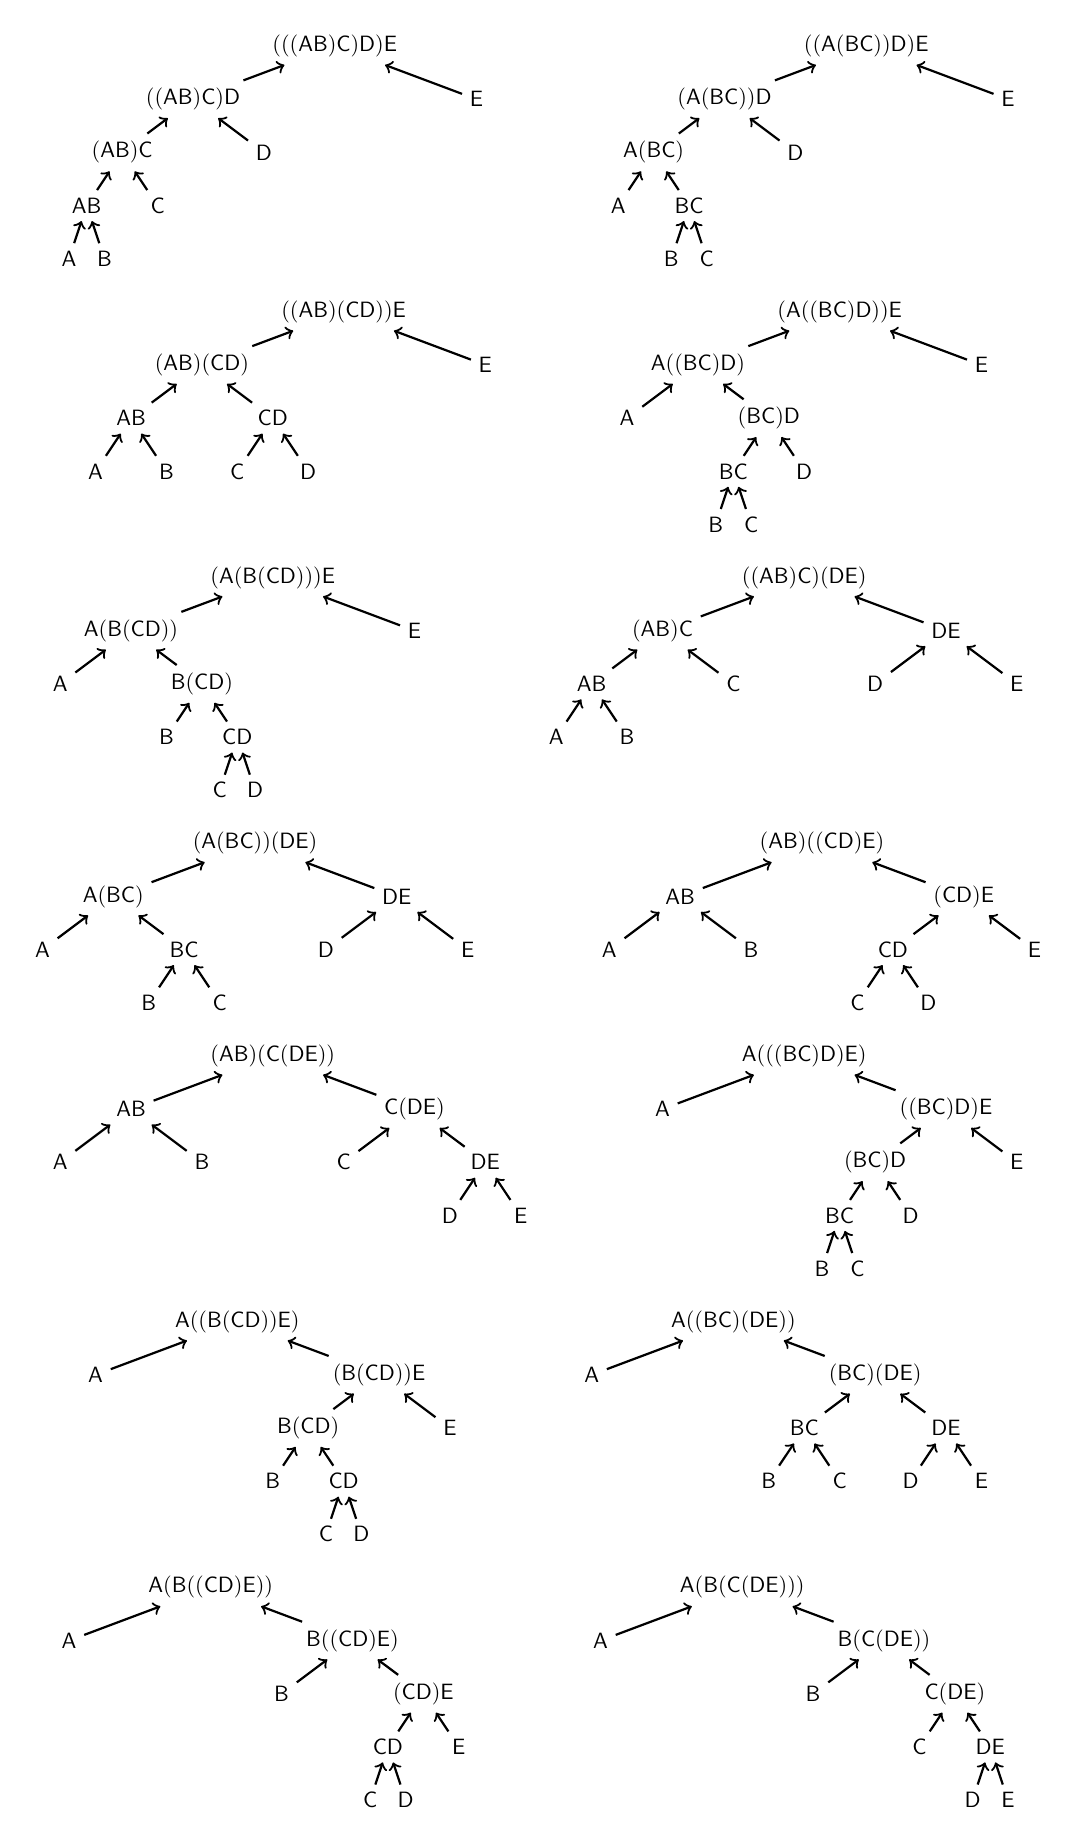
\begin{tikzpicture}[scale=0.9]
  \node[scale=0.8] (536) at (-6.625000,-2.750000) {$\mathsf{A}$};
  \node[scale=0.8] (537) at (-6.125000,-2.750000) {$\mathsf{B}$};
  \node[scale=0.8] (535) at (-6.375000,-2.000000) {$\mathsf{AB}$};
  \node[scale=0.8] (538) at (-5.375000,-2.000000) {$\mathsf{C}$};
  \node[scale=0.8] (534) at (-5.875000,-1.250000) {$\mathsf{(AB)C}$};
  \node[scale=0.8] (539) at (-3.875000,-1.250000) {$\mathsf{D}$};
  \node[scale=0.8] (533) at (-4.875000,-0.500000) {$\mathsf{((AB)C)D}$};
  \node[scale=0.8] (540) at (-0.875000,-0.500000) {$\mathsf{E}$};
  \node[scale=0.8] (532) at (-2.875000,0.250000) {$\mathsf{(((AB)C)D)E}$};
  \path[draw,thick,->] (536) -- (535);
  \path[draw,thick,->] (537) -- (535);
  \path[draw,thick,->] (535) -- (534);
  \path[draw,thick,->] (538) -- (534);
  \path[draw,thick,->] (534) -- (533);
  \path[draw,thick,->] (539) -- (533);
  \path[draw,thick,->] (533) -- (532);
  \path[draw,thick,->] (540) -- (532);
  \node[scale=0.8] (310) at (1.125000,-2.000000) {$\mathsf{A}$};
  \node[scale=0.8] (312) at (1.875000,-2.750000) {$\mathsf{B}$};
  \node[scale=0.8] (313) at (2.375000,-2.750000) {$\mathsf{C}$};
  \node[scale=0.8] (311) at (2.125000,-2.000000) {$\mathsf{BC}$};
  \node[scale=0.8] (309) at (1.625000,-1.250000) {$\mathsf{A(BC)}$};
  \node[scale=0.8] (314) at (3.625000,-1.250000) {$\mathsf{D}$};
  \node[scale=0.8] (308) at (2.625000,-0.500000) {$\mathsf{(A(BC))D}$};
  \node[scale=0.8] (315) at (6.625000,-0.500000) {$\mathsf{E}$};
  \node[scale=0.8] (307) at (4.625000,0.250000) {$\mathsf{((A(BC))D)E}$};
  \path[draw,thick,->] (312) -- (311);
  \path[draw,thick,->] (313) -- (311);
  \path[draw,thick,->] (310) -- (309);
  \path[draw,thick,->] (311) -- (309);
  \path[draw,thick,->] (309) -- (308);
  \path[draw,thick,->] (314) -- (308);
  \path[draw,thick,->] (308) -- (307);
  \path[draw,thick,->] (315) -- (307);
  \node[scale=0.8] (301) at (-6.250000,-5.750000) {$\mathsf{A}$};
  \node[scale=0.8] (302) at (-5.250000,-5.750000) {$\mathsf{B}$};
  \node[scale=0.8] (300) at (-5.750000,-5.000000) {$\mathsf{AB}$};
  \node[scale=0.8] (304) at (-4.250000,-5.750000) {$\mathsf{C}$};
  \node[scale=0.8] (305) at (-3.250000,-5.750000) {$\mathsf{D}$};
  \node[scale=0.8] (303) at (-3.750000,-5.000000) {$\mathsf{CD}$};
  \node[scale=0.8] (299) at (-4.750000,-4.250000) {$\mathsf{(AB)(CD)}$};
  \node[scale=0.8] (306) at (-0.750000,-4.250000) {$\mathsf{E}$};
  \node[scale=0.8] (298) at (-2.750000,-3.500000) {$\mathsf{((AB)(CD))E}$};
  \path[draw,thick,->] (301) -- (300);
  \path[draw,thick,->] (302) -- (300);
  \path[draw,thick,->] (304) -- (303);
  \path[draw,thick,->] (305) -- (303);
  \path[draw,thick,->] (300) -- (299);
  \path[draw,thick,->] (303) -- (299);
  \path[draw,thick,->] (299) -- (298);
  \path[draw,thick,->] (306) -- (298);
  \node[scale=0.8] (498) at (1.250000,-5.000000) {$\mathsf{A}$};
  \node[scale=0.8] (501) at (2.500000,-6.500000) {$\mathsf{B}$};
  \node[scale=0.8] (502) at (3.000000,-6.500000) {$\mathsf{C}$};
  \node[scale=0.8] (500) at (2.750000,-5.750000) {$\mathsf{BC}$};
  \node[scale=0.8] (503) at (3.750000,-5.750000) {$\mathsf{D}$};
  \node[scale=0.8] (499) at (3.250000,-5.000000) {$\mathsf{(BC)D}$};
  \node[scale=0.8] (497) at (2.250000,-4.250000) {$\mathsf{A((BC)D)}$};
  \node[scale=0.8] (504) at (6.250000,-4.250000) {$\mathsf{E}$};
  \node[scale=0.8] (496) at (4.250000,-3.500000) {$\mathsf{(A((BC)D))E}$};
  \path[draw,thick,->] (501) -- (500);
  \path[draw,thick,->] (502) -- (500);
  \path[draw,thick,->] (500) -- (499);
  \path[draw,thick,->] (503) -- (499);
  \path[draw,thick,->] (498) -- (497);
  \path[draw,thick,->] (499) -- (497);
  \path[draw,thick,->] (497) -- (496);
  \path[draw,thick,->] (504) -- (496);
  \node[scale=0.8] (516) at (-6.750000,-8.750000) {$\mathsf{A}$};
  \node[scale=0.8] (518) at (-5.250000,-9.500000) {$\mathsf{B}$};
  \node[scale=0.8] (520) at (-4.500000,-10.250000) {$\mathsf{C}$};
  \node[scale=0.8] (521) at (-4.000000,-10.250000) {$\mathsf{D}$};
  \node[scale=0.8] (519) at (-4.250000,-9.500000) {$\mathsf{CD}$};
  \node[scale=0.8] (517) at (-4.750000,-8.750000) {$\mathsf{B(CD)}$};
  \node[scale=0.8] (515) at (-5.750000,-8.000000) {$\mathsf{A(B(CD))}$};
  \node[scale=0.8] (522) at (-1.750000,-8.000000) {$\mathsf{E}$};
  \node[scale=0.8] (514) at (-3.750000,-7.250000) {$\mathsf{(A(B(CD)))E}$};
  \path[draw,thick,->] (520) -- (519);
  \path[draw,thick,->] (521) -- (519);
  \path[draw,thick,->] (518) -- (517);
  \path[draw,thick,->] (519) -- (517);
  \path[draw,thick,->] (516) -- (515);
  \path[draw,thick,->] (517) -- (515);
  \path[draw,thick,->] (515) -- (514);
  \path[draw,thick,->] (522) -- (514);
  \node[scale=0.8] (526) at (0.250000,-9.500000) {$\mathsf{A}$};
  \node[scale=0.8] (527) at (1.250000,-9.500000) {$\mathsf{B}$};
  \node[scale=0.8] (525) at (0.750000,-8.750000) {$\mathsf{AB}$};
  \node[scale=0.8] (528) at (2.750000,-8.750000) {$\mathsf{C}$};
  \node[scale=0.8] (524) at (1.750000,-8.000000) {$\mathsf{(AB)C}$};
  \node[scale=0.8] (530) at (4.750000,-8.750000) {$\mathsf{D}$};
  \node[scale=0.8] (531) at (6.750000,-8.750000) {$\mathsf{E}$};
  \node[scale=0.8] (529) at (5.750000,-8.000000) {$\mathsf{DE}$};
  \node[scale=0.8] (523) at (3.750000,-7.250000) {$\mathsf{((AB)C)(DE)}$};
  \path[draw,thick,->] (526) -- (525);
  \path[draw,thick,->] (527) -- (525);
  \path[draw,thick,->] (525) -- (524);
  \path[draw,thick,->] (528) -- (524);
  \path[draw,thick,->] (530) -- (529);
  \path[draw,thick,->] (531) -- (529);
  \path[draw,thick,->] (524) -- (523);
  \path[draw,thick,->] (529) -- (523);
  \node[scale=0.8] (489) at (-7.000000,-12.500000) {$\mathsf{A}$};
  \node[scale=0.8] (491) at (-5.500000,-13.250000) {$\mathsf{B}$};
  \node[scale=0.8] (492) at (-4.500000,-13.250000) {$\mathsf{C}$};
  \node[scale=0.8] (490) at (-5.000000,-12.500000) {$\mathsf{BC}$};
  \node[scale=0.8] (488) at (-6.000000,-11.750000) {$\mathsf{A(BC)}$};
  \node[scale=0.8] (494) at (-3.000000,-12.500000) {$\mathsf{D}$};
  \node[scale=0.8] (495) at (-1.000000,-12.500000) {$\mathsf{E}$};
  \node[scale=0.8] (493) at (-2.000000,-11.750000) {$\mathsf{DE}$};
  \node[scale=0.8] (487) at (-4.000000,-11.000000) {$\mathsf{(A(BC))(DE)}$};
  \path[draw,thick,->] (491) -- (490);
  \path[draw,thick,->] (492) -- (490);
  \path[draw,thick,->] (489) -- (488);
  \path[draw,thick,->] (490) -- (488);
  \path[draw,thick,->] (494) -- (493);
  \path[draw,thick,->] (495) -- (493);
  \path[draw,thick,->] (488) -- (487);
  \path[draw,thick,->] (493) -- (487);
  \node[scale=0.8] (471) at (1.000000,-12.500000) {$\mathsf{A}$};
  \node[scale=0.8] (472) at (3.000000,-12.500000) {$\mathsf{B}$};
  \node[scale=0.8] (470) at (2.000000,-11.750000) {$\mathsf{AB}$};
  \node[scale=0.8] (475) at (4.500000,-13.250000) {$\mathsf{C}$};
  \node[scale=0.8] (476) at (5.500000,-13.250000) {$\mathsf{D}$};
  \node[scale=0.8] (474) at (5.000000,-12.500000) {$\mathsf{CD}$};
  \node[scale=0.8] (477) at (7.000000,-12.500000) {$\mathsf{E}$};
  \node[scale=0.8] (473) at (6.000000,-11.750000) {$\mathsf{(CD)E}$};
  \node[scale=0.8] (469) at (4.000000,-11.000000) {$\mathsf{(AB)((CD)E)}$};
  \path[draw,thick,->] (471) -- (470);
  \path[draw,thick,->] (472) -- (470);
  \path[draw,thick,->] (475) -- (474);
  \path[draw,thick,->] (476) -- (474);
  \path[draw,thick,->] (474) -- (473);
  \path[draw,thick,->] (477) -- (473);
  \path[draw,thick,->] (470) -- (469);
  \path[draw,thick,->] (473) -- (469);
  \node[scale=0.8] (381) at (-6.750000,-15.500000) {$\mathsf{A}$};
  \node[scale=0.8] (382) at (-4.750000,-15.500000) {$\mathsf{B}$};
  \node[scale=0.8] (380) at (-5.750000,-14.750000) {$\mathsf{AB}$};
  \node[scale=0.8] (384) at (-2.750000,-15.500000) {$\mathsf{C}$};
  \node[scale=0.8] (386) at (-1.250000,-16.250000) {$\mathsf{D}$};
  \node[scale=0.8] (387) at (-0.250000,-16.250000) {$\mathsf{E}$};
  \node[scale=0.8] (385) at (-0.750000,-15.500000) {$\mathsf{DE}$};
  \node[scale=0.8] (383) at (-1.750000,-14.750000) {$\mathsf{C(DE)}$};
  \node[scale=0.8] (379) at (-3.750000,-14.000000) {$\mathsf{(AB)(C(DE))}$};
  \path[draw,thick,->] (381) -- (380);
  \path[draw,thick,->] (382) -- (380);
  \path[draw,thick,->] (386) -- (385);
  \path[draw,thick,->] (387) -- (385);
  \path[draw,thick,->] (384) -- (383);
  \path[draw,thick,->] (385) -- (383);
  \path[draw,thick,->] (380) -- (379);
  \path[draw,thick,->] (383) -- (379);
  \node[scale=0.8] (479) at (1.750000,-14.750000) {$\mathsf{A}$};
  \node[scale=0.8] (483) at (4.000000,-17.000000) {$\mathsf{B}$};
  \node[scale=0.8] (484) at (4.500000,-17.000000) {$\mathsf{C}$};
  \node[scale=0.8] (482) at (4.250000,-16.250000) {$\mathsf{BC}$};
  \node[scale=0.8] (485) at (5.250000,-16.250000) {$\mathsf{D}$};
  \node[scale=0.8] (481) at (4.750000,-15.500000) {$\mathsf{(BC)D}$};
  \node[scale=0.8] (486) at (6.750000,-15.500000) {$\mathsf{E}$};
  \node[scale=0.8] (480) at (5.750000,-14.750000) {$\mathsf{((BC)D)E}$};
  \node[scale=0.8] (478) at (3.750000,-14.000000) {$\mathsf{A(((BC)D)E)}$};
  \path[draw,thick,->] (483) -- (482);
  \path[draw,thick,->] (484) -- (482);
  \path[draw,thick,->] (482) -- (481);
  \path[draw,thick,->] (485) -- (481);
  \path[draw,thick,->] (481) -- (480);
  \path[draw,thick,->] (486) -- (480);
  \path[draw,thick,->] (479) -- (478);
  \path[draw,thick,->] (480) -- (478);
  \node[scale=0.8] (398) at (-6.250000,-18.500000) {$\mathsf{A}$};
  \node[scale=0.8] (401) at (-3.750000,-20.000000) {$\mathsf{B}$};
  \node[scale=0.8] (403) at (-3.000000,-20.750000) {$\mathsf{C}$};
  \node[scale=0.8] (404) at (-2.500000,-20.750000) {$\mathsf{D}$};
  \node[scale=0.8] (402) at (-2.750000,-20.000000) {$\mathsf{CD}$};
  \node[scale=0.8] (400) at (-3.250000,-19.250000) {$\mathsf{B(CD)}$};
  \node[scale=0.8] (405) at (-1.250000,-19.250000) {$\mathsf{E}$};
  \node[scale=0.8] (399) at (-2.250000,-18.500000) {$\mathsf{(B(CD))E}$};
  \node[scale=0.8] (397) at (-4.250000,-17.750000) {$\mathsf{A((B(CD))E)}$};
  \path[draw,thick,->] (403) -- (402);
  \path[draw,thick,->] (404) -- (402);
  \path[draw,thick,->] (401) -- (400);
  \path[draw,thick,->] (402) -- (400);
  \path[draw,thick,->] (400) -- (399);
  \path[draw,thick,->] (405) -- (399);
  \path[draw,thick,->] (398) -- (397);
  \path[draw,thick,->] (399) -- (397);
  \node[scale=0.8] (281) at (0.750000,-18.500000) {$\mathsf{A}$};
  \node[scale=0.8] (284) at (3.250000,-20.000000) {$\mathsf{B}$};
  \node[scale=0.8] (285) at (4.250000,-20.000000) {$\mathsf{C}$};
  \node[scale=0.8] (283) at (3.750000,-19.250000) {$\mathsf{BC}$};
  \node[scale=0.8] (287) at (5.250000,-20.000000) {$\mathsf{D}$};
  \node[scale=0.8] (288) at (6.250000,-20.000000) {$\mathsf{E}$};
  \node[scale=0.8] (286) at (5.750000,-19.250000) {$\mathsf{DE}$};
  \node[scale=0.8] (282) at (4.750000,-18.500000) {$\mathsf{(BC)(DE)}$};
  \node[scale=0.8] (280) at (2.750000,-17.750000) {$\mathsf{A((BC)(DE))}$};
  \path[draw,thick,->] (284) -- (283);
  \path[draw,thick,->] (285) -- (283);
  \path[draw,thick,->] (287) -- (286);
  \path[draw,thick,->] (288) -- (286);
  \path[draw,thick,->] (283) -- (282);
  \path[draw,thick,->] (286) -- (282);
  \path[draw,thick,->] (281) -- (280);
  \path[draw,thick,->] (282) -- (280);
  \node[scale=0.8] (506) at (-6.625000,-22.250000) {$\mathsf{A}$};
  \node[scale=0.8] (508) at (-3.625000,-23.000000) {$\mathsf{B}$};
  \node[scale=0.8] (511) at (-2.375000,-24.500000) {$\mathsf{C}$};
  \node[scale=0.8] (512) at (-1.875000,-24.500000) {$\mathsf{D}$};
  \node[scale=0.8] (510) at (-2.125000,-23.750000) {$\mathsf{CD}$};
  \node[scale=0.8] (513) at (-1.125000,-23.750000) {$\mathsf{E}$};
  \node[scale=0.8] (509) at (-1.625000,-23.000000) {$\mathsf{(CD)E}$};
  \node[scale=0.8] (507) at (-2.625000,-22.250000) {$\mathsf{B((CD)E)}$};
  \node[scale=0.8] (505) at (-4.625000,-21.500000) {$\mathsf{A(B((CD)E))}$};
  \path[draw,thick,->] (511) -- (510);
  \path[draw,thick,->] (512) -- (510);
  \path[draw,thick,->] (510) -- (509);
  \path[draw,thick,->] (513) -- (509);
  \path[draw,thick,->] (508) -- (507);
  \path[draw,thick,->] (509) -- (507);
  \path[draw,thick,->] (506) -- (505);
  \path[draw,thick,->] (507) -- (505);
  \node[scale=0.8] (209) at (0.875000,-22.250000) {$\mathsf{A}$};
  \node[scale=0.8] (211) at (3.875000,-23.000000) {$\mathsf{B}$};
  \node[scale=0.8] (213) at (5.375000,-23.750000) {$\mathsf{C}$};
  \node[scale=0.8] (215) at (6.125000,-24.500000) {$\mathsf{D}$};
  \node[scale=0.8] (216) at (6.625000,-24.500000) {$\mathsf{E}$};
  \node[scale=0.8] (214) at (6.375000,-23.750000) {$\mathsf{DE}$};
  \node[scale=0.8] (212) at (5.875000,-23.000000) {$\mathsf{C(DE)}$};
  \node[scale=0.8] (210) at (4.875000,-22.250000) {$\mathsf{B(C(DE))}$};
  \node[scale=0.8] (208) at (2.875000,-21.500000) {$\mathsf{A(B(C(DE)))}$};
  \path[draw,thick,->] (215) -- (214);
  \path[draw,thick,->] (216) -- (214);
  \path[draw,thick,->] (213) -- (212);
  \path[draw,thick,->] (214) -- (212);
  \path[draw,thick,->] (211) -- (210);
  \path[draw,thick,->] (212) -- (210);
  \path[draw,thick,->] (209) -- (208);
  \path[draw,thick,->] (210) -- (208);
\end{tikzpicture}

    \caption{৫টা ম্যাট্রিক্সকে গুন করার সবরকম উপায়}
    \label{perfect_binary_trees_with_5_leaves}
  \end{figure}

  ডায়াগ্রামটা যদি একটু ভালোমত দেখো তাহলে খেয়াল করবা আমরা প্রতিটা উপায় জেনারেট
  করার জন্য প্রথমে $ABCDE$ এর মঝে কোন এক জায়গায় ভাগ করেছি, ধরো $B$ আর $C$ এর
  মাঝে ভাগ করলাম, তারপর $AB$ এবং $CDE$ কে যতভাবে গুন করা যায় তা রিকারসিভলি
  হিসাব করেছি। আর এরপর $(AB)$ কে $(CDE)$ এর সাথে গুণ করার জন্য বিবেচনা করেছি।

  সুতরাং আমাদের ডিপি দেখতে এরকম হবেঃ $\DP \two{l}{r} = $ $A_l A_{l+1} A_{l+2}
  \dots A_{r}$ বের করার মিনিমাম কস্ট। বেস কেইসের জন্য $\DP \two{i}{i} = 0$,
  কারণ একটা ম্যাট্রিক্সের গুণফল বের করতে তো কোন অপারেশনই লাগে না। এখন, $l$
  থেকে $r$ ম্যাট্রিক্স গুলোর গুণফল বের করার জন্য আমরা মাঝখানে কোথাও, ধরি $i$
  আর $i+1$ তম ম্যাট্রিক্সের মাঝে ভাগ করলাম, তাহলে আমরা প্রথমে $A_l \dots A_i$
  আর $A_{i+1} \dots A_{r}$ বের করার অপ্টিমাল কস্ট হিসাব করবো, যেটা আমরা
  পাচ্ছি $\DP\two{l}{i}$ এবং $\DP\two{i+1}{r}$ তে। সাথে $(A_l \dots A_{i})
  \times (A_{i+1} \dots A_{r})$ করার কস্ট হলো $N_l M_i M_r$, কারণ $(A_l \dots
  A_{i})$ ম্যাট্রিক্সের এর সাইজ হবে $N_l \times M_i$ আর $(A_{i+1} \dots A_r)$
  ম্যাট্রিক্সের সাইজ হবে $N_{i+1} \times M_r$। সুতরাং $l < r$ এর ক্ষেত্রে
  ডিপির রিকারেন্স হলোঃ
  \[
    \DP\two{l}{r} = \min_{l \le i < r} \DP\two{l}{i} + \DP\two{i+1}{r} + N_l
    M_i M_r
  \]
  ফাইনাল অ্যান্সার হবে $\DP\two{1}{n}$।
\end{solution}

\begin{example}[\href{https://www.spoj.com/problems/MIXTURES/}{SPOJ -
  Mixtures}]
  হ্যারি পটারের সামনে পাশাপাশি একটা সারিতে $n \, (\le 100)$ টা মিশ্রণ সাজানো
  আছে। প্রত্যেকটা মিশ্রণের ১০০টা রঙের মধ্যে একটা রঙ আছে (০ থেক ৯৯ পর্যন্ত
  নাম্বারিং করা), $i$-তম মিশ্রণের রঙ $a_i \, (0 \le a_i \le 99)$। সে সবগুলা
  মিশ্রণকে একসাথে মিশানোর জন্য $n-1$ বার এই অপারেশনটি করবেঃ
  \begin{itemize}
    \item পাশাপাশি ২টা মিশ্রণ নিয়ে তাদের একসাথে মিশিয়ে ২টার মাঝখানে মিশ্রণটা
    রেখে দিবে, অর্থাৎ, বাকি মিশ্রণ গুলোর ক্রমের কোন পরিবর্তন হবে না। পাশাপাশি
    নির্বাচন করা মিশ্রণগুলোর রঙ যদি $x$ এবং $y$ হয়, তাহলে তাদের মিশ্রণের রঙ
    হবে $(x+y) \mod 100$\footnote{এখানে $a \mod m$ দিয়ে $a$ কে $m$ দিয়ে ভাগ
    করলে যেই ভাগশেষ থাকে তা বুঝানো হচ্ছে।}। আর তাদের মিশ্রিত করার সময় $xy$
    পরিমাণের ধোঁয়া উৎপন্ন হয়।
  \end{itemize}
  তোমাকে বের করতে হবে সবচাইতে কম কতো পরিমাণের ধোঁয়া উৎপন্ন করে মিশ্রণ গুলোকে
  হ্যারি মিশ্রিত করতে পারবে।
\end{example}

\begin{solution}
  আগের প্রবলেমের মতই এই প্রবলেমেও $n$টা মিশ্রণকে মিক্স করার যেকোনো উপায়কেই
  তুমি একটা $n$ লিফের পারফেক্ট বাইনারি ট্রি হিসেবে আঁকতে পারবা।
  $\DP\two{l}{r}$ হলো $l$ থেকে $r$ এর মধ্যে মিশ্রণ গুলোকে যদি অপ্টিমালি
  মিশানো হয়, তাহলে সর্বনিম্ন কি পরিমাণের ধোঁয়া উৎপন্ন হবে। এখন তুমি মাঝখানে
  কোথায় ভাঙ্গবে তার উপর ইটারেট করবা। ধরো, $i$ আর $i+1$ এর মাঝে ভাঙ্গেছো,
  তাহলে ২ পাশের কস্ট হলো $\DP\two{l}{i}$ আর $\DP\two{i+1}{r}$। $l \ldots i$
  এর মিশ্রণগুলোকে মিক্স করে যেই মিশ্রণ পাবো তার রঙ হবে $\left(\sum_{j=l}^{i}
  a_j \right) \mod 100$ (কারণ, $(((x+y)\mod m) + z) \mod m = (x+y+z) \mod
  m$)। একইভাবে $i+1 \ldots r$ এর মিশ্রণগুলোকে মিক্স করার পর $\left(
  \sum_{j=i+1}^{r} a_j \right) \mod 100$ রঙের মিশ্রণ পাবা। এদের মিক্স করলে
  আবার $\left( \left(\sum_{j=l}^{i} a_j \right) \mod 100 \right) \times
  \left( \left( \sum_{j=i+1}^{r} a_j \right) \mod 100 \right)$ পরিমাণের ধোঁয়া
  উৎপন্ন হবে। তাহলে রিকারেন্সটা হলোঃ
  \[
    \DP\two{l}{r} = \min_{i=l}^{r-1} \DP\two{l}{i} + \DP\two{i+1}{r} + L
    \times R
  \]
  যেখানে, $L = \left(\sum_{j=l}^{i} a_j \right) \mod 100$, $R = \left(
  \sum_{j=i+1}^{r} a_j \right) \mod 100$, এবং $\DP\two{i}{i} = 0$।
\end{solution}

\begin{example}[\href{http://www.usaco.org/index.php?page=viewproblem2&%
  cpid=972}{USACO - Greedy Pie Eaters}]
  ফার্মার জনের কাছে $M$টা গরু আর $N$ টা পাই আছে। গরুগুলো $1$ থেকে $M$ এবং
  পাইগুলো $1$ থেকে $N$ পর্যন্ত নাম্বারিং করা। $i$-তম গরু $[l_i, r_i]$ রেঞ্জের
  মধ্যে পাইগুলো খেতে পছন্দ করে। তোমাকে আরেকটা জিনিস বলে দেওয়া আছে, তা হলো ২টা
  গরুর পছন্দের রেঞ্জ একই হবে না কখনো। $i$-তম গরুর ওজন হলো $w_i$।

  \noindent ফার্মার জন একটা সিকুয়েন্স $c_1, c_2, \ldots, c_K$ বাছাই করবে,
  যেটা দিয়ে গরুগুলো কি অর্ডারে পাই খেতে আসবে তা বুঝাবে, অর্থাৎ, প্রথমে
  $c_1$-তম গরুটি আসবে, এরপর $c_2$-তম গরুটি আসবে...। একটা গরু আসলে সে তার
  পছন্দের রেঞ্জে বাকি থাকা সব পাই খেয়ে ফেলবে। কিন্তু যদি তার পছন্দের রেঞ্জে
  কোন পাইই বাকি না থাকে তাহলে সে মন খারাপ করে বসবে! ফার্মার জন এমন একটা
  সিকুয়েন্স বাছাই করতে চায় যাতে $(w_{c_1} + w_{c_2} + \ldots + w_{c_K})$ এর
  মান ম্যাক্সিমাইজ হয়, এবং বাছাই করা $K$ টা গরুর মধ্যে কেও মন খারাপ না করে।
  $1 \le N \le 300, 1 \le M \le \frac{N(N+1)}{2}, 1 \le w_i \le 10^6$।
\end{example}

\begin{example}[\href{https://codeforces.com/contest/1146/problem/%
  G}{Codeforces 1146G - Zoning Restrictions}]
  তুমি $n$ টা বিল্ডিং বানাবে, এবং বিল্ডিং বানানোর স্পটগুলো $1$ থেকে $n$
  পর্যন্ত নাম্বারিং করা। প্রতিটা বিল্ডিঙের উচ্চতা 0 থেকে $h$ এর মধ্যে যেকোনো
  একটি পর্ণসংখ্যা হতে পারে। কোন স্পটে যদি $a$ উচ্চতার বিল্ডিং বানাও তাহলে
  তুমি $a^2$ টাকা পাবা। তুমি যাতে ইচ্ছা মতো উচ্চতার বিল্ডিং নির্মাণ করতে না
  পারো তাই $m$ টা শর্ত দেওয়া আছে -- $i$ তম শর্তে তোমাকে বলা আছে $l_i$ থেকে
  $r_i$ স্পটের বিল্ডিং গুলোর উচ্চতা সর্বোচ্চ $x_i$ হতে পারবে। যদি এদের মধ্যে
  কোনটার উচ্চতা $x_i$ এর বেশি হয় তাহলে তোমাকে $c_i$ টাকা পেনাল্টি দিতে হবে।
  খেয়াল করো, $l_i$ থেকে $r_i$ এর মধ্যে একাধিক বিল্ডিং-এর উচ্চতা $x_i$ এর
  চাইতে বেশি হলেও কিন্তু $i$-তম শর্ত ভঙ্গের জন্য একবারই $c_i$ টাকা পেনাল্টি
  দিবে। অপ্টিমালভাবে বিল্ডিং-এর উচ্চতা নির্বাচন করে ম্যাক্সিমাম কতো প্রফিট
  পেতে পারো তা হিসাব করো। $1 \le n, m, h \le 50, 1 \le l_i \le r_i \le n, 0
  \le x_i \le h, 1 \le c_i \le 5\,000$।
\end{example}

\begin{example}[\href{http://www.usaco.org/index.php?page=viewproblem2%
  &cpid=698}{USACO - Subsequence Reversal}]
  তোমাকে একটা অ্যারে $a_1, a_2, \ldots, a_N$ দেওয়া আছে। প্রথমে এই অ্যারের
  একটি সাবসিকুয়েন্স নির্বাচন করে তা রিভার্স করবা, এবং এরপর যেই অ্যারেটা পাবা
  তার Longest Non-decreasing সাবসিকুয়েন্স বের করবা। তোমার উদ্দেশ্য হচ্ছে, যেই
  সাবসিকুয়েন্সটা রিভার্স করবা, সেটা এমনভাবে নির্বাচন করা, যাতে Longest
  Non-decreasing সাবসিকুয়েন্স সর্বোচ্চ হয়। যেমন, নিচের অ্যারেটির গাড় করা
  সাবসিকুয়েন্স নির্বাচন করে সেটি রিভার্স করলে পুরো অ্যারেটিই Non-decreasing
  হয়ে যায়। $1 \le N, a_i \le 50$।
  \begin{center}
    \begin{tabular}{|c|c|c|c|c|c|c|c|c|}
      \hline
      1 & 2 & 3 & \cellcolor{black!25}9 & 5 & 6 & \cellcolor{black!25}8 &
      \cellcolor{black!25}7 & \cellcolor{black!25}4 \\
      \hline
    \end{tabular}\\
    $\downarrow$\\
    \begin{tabular}{|c|c|c|c|c|c|c|c|c|}
      \hline
      1 & 2 & 3 & \cellcolor{black!25}4 & 5 & 6 & \cellcolor{black!25}7 &
      \cellcolor{black!25}8 & \cellcolor{black!25}9 \\
      \hline
    \end{tabular}
  \end{center}
\end{example}

\begin{example}[\href{https://codeforces.com/contest/1107/problem/E}%
  {Codeforces 1107E - Vasya and Binary String}]
  তোমার কাছে $n$ লেংথের একটি বাইনারি স্ট্রিং $s$, এবং $n$ সাইজের একটি অ্যারে
  $a$ আছে। স্ট্রিংটা খালি না হয়ে যাওয়া পর্যন্ত তুমি এই অপারেশনটি অ্যাপ্লাই
  করবাঃ $s$ এর মধ্যে একটা কন্সেকিউটিভ সাবস্ট্রিং বাছাই করবা যাতে সেই
  সাবস্ট্রিং এর সব ক্যারেক্টার একই হয়, এবং সেই সাবস্ট্রিংটা ডিলিট করে এরপর ২
  পাশের বাকি থাকা সাবস্ট্রিংগুলো (এগুলোর কোনটা ফাকা হলে সমস্যা নেই) জোড়া
  লাগিয়ে দিবা। যেমন 1\colorbox{black!25}{111}101 $\rightarrow$ 1101। $x$
  লেংথের সাবস্ট্রিং ডিলিট করলে $a_x$ পয়েন্ট পাবে। ম্যাক্সিমাম কতো পয়েন্ট
  পেতে পারো তুমি? $1 \le n \le 100, 1 \le a_i \le 10^9$।
\end{example}

\begin{example}[\href{https://atcoder.jp/contests/arc104/tasks/arc104_f}%
  {AtCoder - Visibility Sequence}]
  আগের বিল্ডিং বানানোর ঠিকাদারিতে তুমি ব্যাপক পরিমাণের লাভ করেছ (ডাইনামিক
  প্প্রোগ্রামিংকে ধন্যবাদ না দিলেই নয়), তাই তুমি আবারো পরিকল্পনা করেছ $N$ টা
  বিল্ডিং বানাবে। এইবারের শর্তগুলো হলো, প্রতিটা $i \, (1 \le i \le N)$ এর
  জন্য তোমাকে একটা $X_i$ দেয়াও আছে, যার মানে হলো $i$ তম বিল্ডিংয়ের উচ্চতা 1
  থেকে $X_i$ এর মধ্যে যেকোনো একটি পুর্ণসংখ্যা হতে পারবে। ধরো তুমি $i$ তম
  বিল্ডিং বানিয়েছ $H_i$ উচ্চতার। এখন প্রতি $i \, (1 \le i \le N)$ এর জন্য
  আমরা $P_i$ কে এভাবে ডিফাইন করবোঃ যদি এমন কোন পর্ণসংখ্যা $j \, (1 \le j <
  i)$ থাকে যাতে $H_j > H_i$ হয়, তাহলে $P_i$ হবে এমন ম্যাক্সিমাম $j$, আর নাহলে
  $P_i = -1$। এবার $H$ সিকুয়েন্সটির সবরকম কম্বিনেশনের কথা চিন্তা করো, তারা
  প্রত্যেকেই একটি করে $P$ জেনারেট করবে। দুটি ভিন্ন $H$ এর জন্য তাদের জেনারেট
  করা $P$ একই হয়ে যেতে পারে আবার ভিন্নও হতে পারে। তোমাকে বের করতে হবে, কয়টা
  ভিন্ন ভিন্ন $P$ জেনারেট হবে। $1 \le N \le 100, 1 \le X_i \le 10^5$।
\end{example}

\begin{example}[\href{https://codeforces.com/gym/102979/problem/G}%
  {XXI Open Cup, GP of Suwon - Generate The Array}]
  ধরো তোমাকে একটা $N$ লেংথের অ্যারে $A$ দেওয়া আছে, এবং তুমি এতে কিছু কুয়েরি
  করবাঃ অ্যারের একটা সেগমেন্ট $[i, j]$ এর জন্য সেই সেগমেন্টের ম্যাক্সিমাম বের
  করবা। $[i, j]$ সেগমেন্টটি $Q_{i, j}$ বার করা হবে।\\
  কিন্তু অ্যারেটা তোমাকে দেওয়া নাই, তুমি বানাবে সেটা। $1$ থেকে $N$ এর মধ্যে
  প্রতিটা $i$ এর জন্য $A_i$ এর মান হিসেবে তুমি $K_i$ টা আলাদা আলাদা মান
  $V_{i,1}, V_{i,2}, \ldots, V_{i, K_i}$ থেকে একটি বাছাই করতে পারবা। $A_i$ এর
  জন্য $V_{i, j}$ বাছাই করার কস্ট হলো $C_{i, j}$।\\
  সবগুলো কুয়েরির শেষে তোমার স্কোর হবেঃ (সব ইন্টারভাল কুয়েরির রেজাল্টের যোগফল)
  $-$ ($A_i$ ভ্যালু গুলা বাছাই করার কস্টের যোগফল)। ম্যাক্সিমাম কতো স্কোর পেতে
  পারো তা বের করো।
\end{example}